\documentclass[]{article}
\usepackage[utf8]{inputenc}
\usepackage{cite}
\usepackage{amsmath,amssymb,amsfonts}
\usepackage{algorithmic}
\usepackage{graphicx}
\usepackage{textcomp}
\usepackage{xcolor}
\usepackage{multicol}
\usepackage{cuted}
\usepackage{caption}
\usepackage{subcaption}
\usepackage{hyperref}

\hypersetup{
    colorlinks=true,
    linkcolor=blue,
    filecolor=magenta,      
    urlcolor=cyan}

\title{ENPM667\textemdash Control of Robotic Systems \\ Project~1: Unscented Kalman Filter}
\author{{Trevian~Jenkins} \\
    {\textit{Maryland Applied Graduate Engineering}} \\
    {\textit{University of Maryland, College Park}} \\
    {College Park, Maryland, USA} \\
    {trj0011@umd.edu}
\\ \\
    {Markose~Jacob} \\
    {\textit{Maryland Applied Graduate Engineering}} \\
    {\textit{University of Maryland, College Park}} \\
    {College Park, Maryland, USA} \\
    {markj11@umd.edu}}
\date{27 November 2020}

%\def\BibTeX{{\rm B\kern-.05em{\sc i\kern-.025em b}\kern-.08em
%    T\kern-.1667em\lower.7ex\hbox{E}\kern-.125emX}}

\begin{document}

\maketitle
\thispagestyle{empty}

\begin{abstract}
The Kalman filter is a widely-used technique for extracting  meaningful information out of input data in the presence of disturbances. While the Kalman filter succeeds in situations where the system model is linear, it fails to approximate the true data correctly beyond the range of linearity. The extended Kalman filter provides a generalization of the Kalman filter for use in nonlinear systems, and it performs well when the disturbance is normally distributed, which is usually assumed.  However, the extended Kalman filter suffers from bias when the data falls under some other statistical distribution. Such a change in distribution may for example occur, as we will see, from switching from polar to Cartesian coordinates. The unscented Kalman filter circumvents this issue by transforming the distribution along with the data. This report summarizes our implementation of the unscented Kalman filter and describes its advantage over the linear and extended Kalman filters, as well as plotting some examples.
\end{abstract}

\newpage

\thispagestyle{empty}
\tableofcontents
\listoffigures

\newpage

\section{Introduction}
The Kalman filter was popularized by Rudolf Kalman in 1960, and it has become the \textit{de facto} standard of statistical estimation and prediction when dealing with data that contains disturbances, such as that of robotic sensors. In a linear system, or a subset of data that can be linearized within a certain domain, the basic linear Kalman filter can sufficiently estimate the true data. However, when the system is generally nonlinear, the standard Kalman filter quickly loses accuracy when estimating the values of state variables. Thus, we seek to use a generalization the Kalman filter for use in nonlinear systems.

We referred to "New extension of the Kalman filter to nonlinear systems," by Julier and Uhlmann, to implement the unscented Kalman filter. In this report, we will first describe the mathematical theory behind the linear, extended, and unscented Kalman filters. We will use a simple sinusoidal example to illustrate the unscented Kalman filter in use. We will also replicate Fig. 1 and the space vehicle trajectory example from the paper to show the practical use of the unscented Kalman filter.

\section{Mathematical Theory}

\subsection{Linear Kalman Filter}

Let us first look at the standard Kalman filter, or the \textit{linear} Kalman Filter. When using the Kalman filter, we desire to regularly update our estimation of the state variables based on the previous estimation of the state variables, the uncertainty of the accuracy of our current state vector, and the interval of time $\Delta t_{P}$ between predictions. Every time the value of the state vector is predicted, the uncertainty, which is stored in a covariance matrix $\boldsymbol{P}$, grows, due to the fact that we are effectively extrapolating the current position since any information was last received. We will use the example of a sine wave to illustrate. The equations of motion we will use for this example are as follows:

\begin{equation}
x(t) = \alpha\sin{\omega t} + \beta\cos{\omega t}
\label{equ:eom1}
\end{equation}
\begin{equation}
\cfrac{d}{dt} x(t) = \dot{x}(t) = \alpha\omega\cos{\omega t} - \beta\omega\sin{\omega t} \\
\label{equ:eom2}
\end{equation}
\begin{equation}
\cfrac{d^{2}}{dt^{2}} x(t) = \ddot{x}(t) = -\alpha\omega^{2}\sin{\omega t} - \beta\omega^{2}\cos{\omega t} \\
\label{equ:eom3}
\end{equation}

We may linearize equations (\ref{equ:eom1}) through (\ref{equ:eom3}) by using the small angle approximation as follows. If the value of $x$ is assumed to be small (\textless \ 0.2 rad), then $\sin{x} \approx x$. The small angle approximation is derived from the Maclaurin series approximation:
\[ f(x) = \sum_{k=0}^{\infty}{\frac{x^{k}f^{(k)}(x)}{k!}} \]
The Maclaurin series for the sine function is
\[\begin{split}
\sin{x} & = \sum_{k=0}^{\infty}{(-1)^{k} \cfrac{x^{2k + 1}}{(2k + 1)!}} \\
        & = x - \frac{x^{3}}{6} + \frac{x^{5}}{120} - \frac{x^{7}}{5040} + \dots \\
        & \approx x,
\end{split}\]
with the final approximation neglecting higher-order terms. A similar derivation is used to approximate the cosine function as
\[\begin{split}
\cos{x} & = \sum_{k=0}^{\infty}{(-1)^{k} \cfrac{x^{2k}}{(2k)!}} \\
        & = 1 - \frac{x^{2}}{2} + \frac{x^{4}}{24} - \frac{x^{6}}{720} + \dots \\
        & \approx 1 - \frac{x^{2}}{2}.
\end{split}\]
For the linear Kalman filter, it is necessary that we make the slightly less accurate, but still reasonable approximation,
\[\begin{split}
\cos{x} \approx 1.
\end{split}\]
This linear approximation is reasonable for many applications and is a precursor for the use of the linear Kalman filter. With the small-angle approximation, the equations of motion then become
\begin{equation}
\begin{split}
x(t) & \approx \alpha t + \beta \\
\dot{x}(t) & \approx \alpha\omega - \beta\omega t \\
\ddot{x}(t) & \approx -\alpha\omega^{2} t - \beta\omega^{2} \approx -\omega^{2}x
\end{split}.
\label{equ:eom_linear}
\end{equation}

Using our equations of motion and the small angle approximation, we may define the state vector $\boldsymbol{x}$ as
\begin{equation}
\boldsymbol{x} = \begin{bmatrix} x_{1} \\ x_{2} \end{bmatrix}
                    = \begin{bmatrix} x \\ \dot{x} \end{bmatrix}.
\label{equ:state_variables}
\end{equation}

The state transition matrix $A$ may then be defined as follows:
\begin{equation}
\boldsymbol{A} = \begin{bmatrix} 1 & \Delta t \\
                -\omega^{2}\Delta t & 1 \end{bmatrix}
\label{equ:a_lkf}
\end{equation}

The measurement matrix $\boldsymbol{H}$ describes the relation between a new measurement $z$ and the state vector $\boldsymbol{x}$. For example, if we have a system that is capable of measuring $x$ but not $\dot{x}$, then $h$ would be $\begin{bmatrix} 1 & 0 \end{bmatrix}$.

With equations (\ref{equ:state_variables}) and (\ref{equ:a_lkf}), we find that the next (\textit{a priori}) values of the state vector and covariance matrix are predicted to be
\begin{equation}
\begin{split}
\boldsymbol{x}_{n}^{-} & = \boldsymbol{A} x_{n-1} \\
\boldsymbol{P}_{n}^{-} & = \boldsymbol{A}\boldsymbol{P}_{n-1}\boldsymbol{A}^{T} + \boldsymbol{Q},
\end{split}
\label{equ:state_predict_lkf}
\end{equation}
where $\boldsymbol{Q}$ is the covariance matrix describing the process noise (from random disturbances, etc.). When new data is received, the measurement step updates $\boldsymbol{x}$ and $\boldsymbol{P}$ as follows:
\begin{equation}
\begin{split}
\boldsymbol{K}_{n} & = \boldsymbol{P}_{n}^{-} \boldsymbol{H}^{T}
(\boldsymbol{H} \boldsymbol{P}_{n}^{-} \boldsymbol{H}^{T}
+ \boldsymbol{R})^{-1} \\
\boldsymbol{x}_{n} & = \boldsymbol{x}_{n}^{-} + \boldsymbol{K}_{n} (z_{n} - H\boldsymbol{x}_{n}^{-}) \\
\boldsymbol{P}_{n} & = (\boldsymbol{I} - \boldsymbol{K}_{n}\boldsymbol{H}) \boldsymbol{P}_{n}^{-}
\end{split}.
\label{equ:state_measure_lkf}
\end{equation}

\subsection{Extended Kalman Filter}

In the case of the extended Kalman filter, we run the prediction and measurement steps as before. The major change, however, is that instead of using matrices to define the state transitions, we simply use a vector function. Equations (\ref{equ:eom1}) through (\ref{equ:eom3}) dictate that the next (\textit{a priori}) value of the state vector is predicted to be
\begin{equation}
\begin{split}
\boldsymbol{x}_{n}^{-} & = f(\boldsymbol{x}_{n-1}) \\
& = \begin{bmatrix} f_{1}(x_{1}, x_{2}) \\
                    f_{2}(x_{1}, x_{2}) \end{bmatrix} \\
& = \begin{bmatrix} x_{1} + x_{2} \Delta t \\ 
                    x_{2} -\omega^{2} x_{1} \Delta t \end{bmatrix},
\end{split}
\label{equ:state_predict_ekf}
\end{equation}
and when this prediction is made, the uncertainty matrix becomes
\begin{equation}
\boldsymbol{P}_{n}^{-} = \boldsymbol{A}_{n} \boldsymbol{P}_{n-1} \boldsymbol{A}_{n}^{T}
                       + \boldsymbol{W}_{n} \boldsymbol{Q}_{n-1} \boldsymbol{W}_{n}^{T},
\label{equ:uncertainty_predict}
\end{equation}
where $\boldsymbol{A}$ is the Jacobian matrix
\[ \boldsymbol{A}_{ij} = \cfrac{\partial f_{i}}{\partial x_{j}}(\boldsymbol{x}_{n-1}), \]
$\boldsymbol{Q}$ is the covariance matrix describing the process noise $w$, and $\boldsymbol{W}$ is the Jacobian matrix 
\[ \boldsymbol{W}_{ij} = \cfrac{\partial f_{i}}{\partial w_{j}}(\boldsymbol{x}_{n-1}). \]

The function $h(\boldsymbol{x})$ describes the relation between a new measurement $z$ and the state vector $\boldsymbol{x}$. Whenever new measurements are retrieved, such as azimuth information in our case, the next (\textit{a posteriori}) value of the state matrix is updated to be
\begin{equation}
\label{equ:state_measure}
\boldsymbol{x}_{n} = \boldsymbol{x}_{n}^{-} + \boldsymbol{K}_{n}[z_{n}
- h(\boldsymbol{x}_{n}^{-})],
\end{equation}
where
\[ \boldsymbol{K}_{n} = \boldsymbol{P}_{n}^{-} \boldsymbol{H}_{n}^{T}
(\boldsymbol{H}_{n} \boldsymbol{P}_{n} \boldsymbol{H}_{n}^{T}
+\boldsymbol{V}_{n} \boldsymbol{R}_{n} \boldsymbol{V}_{n}^{T})^{-1}, \]
$\boldsymbol{H}$ is the Jacobian matrix
\[ \boldsymbol{H}_{ij} = \cfrac{\partial h_{i}}{\partial x_{j}}(\boldsymbol{x}_{n}), \]
$\boldsymbol{R}$ is the covariance matrix describing the measurement noise $v$, and $\boldsymbol{V}$ is the Jacobian matrix 
\[ \boldsymbol{V}_{ij} = \cfrac{\partial h_{i}}{\partial v_{j}}(\boldsymbol{x}_{n}). \]
With the arrival of new measurements, uncertainty always decreases, and the new uncertainty matrix $\boldsymbol{P}$ becomes
\begin{equation}
\boldsymbol{P}_{n} = (\boldsymbol{I} - \boldsymbol{K}_{n} \boldsymbol{H}_{n}) \boldsymbol{P}_{n}^{-}.
\label{equ:uncertainty_measure}
\end{equation}

The ($-$) superscript in the $\boldsymbol{x}^{-}$ vector and $\boldsymbol{P}^{-}$ matrices indicate that those values are \textit{a priori} values that were calculated from the predict step, before the arrival of measurement data. We repeat the cycle of obtaining measurements of the current state vector and using those measurements to infer about the next values of the state vector. The output of the Kalman filter provides an improved estimate over the raw sensor data, which is to be used as e.g. the feedback within a control system, or for visualization.

\subsection{Complex-Step Derivative Approximation}

We utilized the method described in this section to compute the Jacobian matrices for the Kalman filter. Traditionally, the derivative of a function $f(x)$ is estimated using the finite difference approximation
\begin{equation}
\label{equ:derivative_approx}
f'(x) \approx \frac{f(x+h) - f(x)}{h}
\end{equation}
for, say, a small stepsize $h \approx 10^{-7}$. However, we wish to avoid cancellation error arising from taking differences of such small values. Thus, the partial derivatives of the aforementioned Jacobian functions are computed using the complex-step derivative approximation described as follows. The derivative of $f(x)$ with respect to $x$ is calculated as
\begin{equation}
\cfrac{\partial f}{\partial x} = \cfrac{\Im [f(x + ih)]}{h},
\label{equ:complex_step}
\end{equation}
where $\Im [z]$ returns the imaginary part of the complex number $z$. The complex step method results from the Taylor series approximation about a real point x:
\begin{equation}
f(x + ih) = f(x) + ihf'(x) - \frac{h^{2}f''(x)}{2!} - \frac{ih^{3}f'''(x)}{3!} + \cdots
\label{equ:complex_step_taylor}
\end{equation}
Taking the imaginary part of equation (\ref{equ:complex_step_taylor}) and dividing by $h$ results in
\begin{equation}
\begin{split}
f'(x) & = \frac{\Im [f(x + ih)]}{h} + \frac{h^{2}f'''(x)}{3!} + \frac{h^{4} f^{(5)}(x)}{5!} + \cdots \\
      & = \frac{\Im [f(x + ih)]}{h} + \mathcal{O}(h^{2}) \\
      & \approx \frac{\Im [f(x + ih)]}{h}.
\end{split}
\label{equ:complex_step_approx}
\end{equation}
The final result truncates the higher-order terms, giving a truncation error $\mathcal{O}(h^{2})$. Since this calculation does not involve a subtraction operation, it is not prone to cancellation errors resulting from subtractions. Therefore, we consider the complex step method superior to the more traditional derivative approximation in equation (\ref{equ:derivative_approx}) for small stepsize $h$, hence our use in the extended Kalman filter.

\subsection{Unscented Kalman Filter}

The basic setup of the unscented Kalman filter is similar to the extended kalman filter. We still run the prediction and measurement steps as we always have. However, we now implement what is known as an \textit{unscented transformation}. This operation transforms the mean and covariance information about a distribution along with the data itself.

The following steps are performed to make this transformation happen:
\begin{enumerate}
    \item Creating the sigma points through a sigma point selection algorithm.
    \item Calculating the transformed set:
        \[\hat{x}_{a,n} = f[x_{a,n}]\]
    \item Predicting the mean:
        \[\hat{\mu}_{a,n} = \sum_{i=0}^{p}{W^{(i)} \hat{x}_{a,n}^{(i)}}\]
    \item Predicting the covariance:
        \[\hat{K}_{a,n} = \sum_{i=0}^{p}{W^{(i)} (\hat{x}_{a,n}^{(i)} - \hat{\mu}_{a,n})(\hat{x}_{a,n}^{(i)} - \hat{\mu}_{a,n})^{T} }\]
    \item Instantiating prediction points:
        \[y_{n}^{(i)} = g[x_{a,n}^{(i)}]\]
    \item Predicting the observation:
        \[y_{n} = g[y_{n}^{(i)}]\]
    \item Calculating the innovation covariance:
        \[\hat{S}_n = \sum_{i=0}^{p}{W^{(i)} (\hat{y}_{n}^{(i)} - \hat{y}_n)(\hat{y}_{n}^{(i)} - \hat{y}_n)^{T} }\]
    \item Calculating the cross covariance matrix:
        \[\hat{K}^{xy}_{n} = \sum_{i=0}^{p}{W^{(i)} (\hat{x}_{n}^{(i)} - \hat{\mu}_n)(\hat{x}_{n}^{(i)} - \hat{\mu}_n)^{T} }\]
    \item The update is performed as per the typical Kalman filter operation:
        \[\begin{split}
        \mu_{n} & = \hat{\mu}_{n} + W_{n}\nu_{n} \\
        K_{n} & = \hat{K}_{n} - W_{n} \hat{S}_{n} W_{n}^{T} \\
        \nu_{n} & = y_{n} - \hat{y}_{n} \\
        W_{n} & = \hat{K}^{xy}_{n} \hat{S}_{n}^{-1}
        \end{split}\]
\end{enumerate}

From step (9) above, we obtain our new \textit{a posteriori} estimate of the mean value of the state vector $\mu_{n}$ and error covariance matrix $K_{n}$.

\section{Results}

\subsection{Example Sinusoidal Wave}
\label{sec:sine}

The results we achieved are as follows. From our sinusoidal example described before, we illustrate the true curve and the filtered data in Fig. \ref{fig:ukf_sine}. The true value of the wave, the measurements, and the filtered value of the wave are indicated in the plot, with the filtered value of the wave at any given time instant $t$ in reasonable correspondence with the true value at that time.

\begin{figure}[t]
\centerline{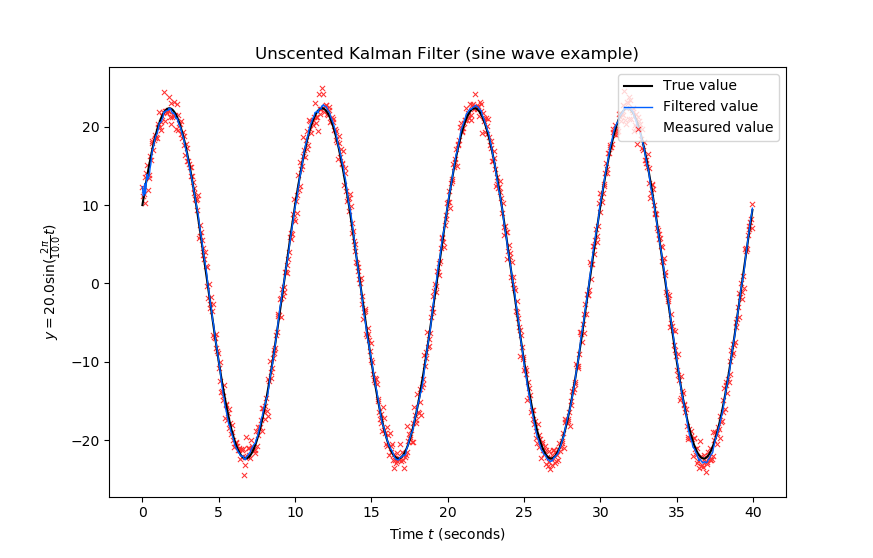
\includegraphics[height=6cm]{sine_example.png}}
\caption{Unscented Kalman filter for sinusoidal wave.}
\label{fig:ukf_sine}
\end{figure}

\subsection{Coordinate System Conversion}
\label{sec:cart_polar}

To illustrate the effects on nonlinear transformation, we will show the transformation of data points representing location data from a sensor tracking a target placed at $(x, y)$ coordinates (0, 1). The sensor used in the example from the original paper returned a mean radius of 1.0 m, with a standard deviation of 0.02 m. The mean angle returned by the sensor was $\frac{\pi}{2}$ rad, while the standard deviation of the angle was $\frac{\pi}{20}$ rad. This data was converted into Cartesian coordinates as
\begin{equation}
\begin{split}
x & = r\cos{\theta} \\
y & = r\sin{\theta}
\end{split}
\label{equ:polar_to_cartesian}
\end{equation}
The data points are plotted in the left plot, and the irregular distribution resulting from the coordinate transformation is apparent.

On the right are plots containing the statistical information contained within the data. The x symbol indicates the true mean of the data, and the dashed ellipse is the true covariance ellipse. The linearized version of the sensor data has a mean indicated by the o symbol, and the dotted ellipse is the corresponding covariance ellipse. As one can see, the data after a linearization suffers from bias created by the linearization of the data points without transforming the statistical data as well.

\begin{figure}[ht!]
\centering\noindent
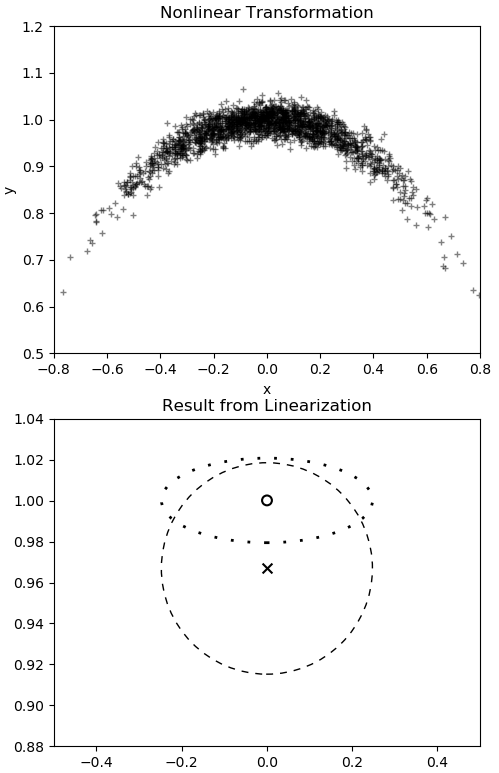
\includegraphics[width=0.7\textwidth]{fig_1.png}
\captionof{figure}{Transformation of coordinates from polar to Cartesian, and the effect on the mean and covariance.}
\label{fig:cart_polar}
\end{figure}

\subsection{Vehicular Trajectory Example}
\label{sec:vehicle}

For the practical example we decided to illustrate, we attempted to replicate the results of Section VI\textemdash \textquotedblleft Applying the UT to Recursive Estimation\textquotedblright\textemdash from the original paper by Julier and Uhlmann\cite{b1}. This section details the estimation of the state of a vehicle as it is reentering Earth's atmosphere. The vehicle is being observed by a radar on Earth's surface, near the projected landing location.

The following state variables are tracked by the filter:
\begin{itemize}
    \item $x_{1}$: The $x$-component of the position of the vehicle
    \item $x_{2}$: The $y$-component of the position of the vehicle
    \item $x_{3}$: The $x$-component of the velocity of the vehicle
    \item $x_{4}$: The $y$-component of the velocity of the vehicle
    \item $x_{5}$: The aerodynamic coefficient, which is a property of the aerodynamics of the vehicle
\end{itemize}

The vehicle has the following state dynamics:
\begin{equation}
\begin{split}
    \dot{x}_{1}(k) & = x_{3}(k) \\
    \dot{x}_{2}(k) & = x_{4}(k) \\
    \dot{x}_{3}(k) & = D(k) x_{3}(k) + G(k) x_{1}(k) + v_{1}(k) \\
    \dot{x}_{4}(k) & = D(k) x_{4}(k) + G(k) x_{2}(k) + v_{2}(k) \\
    \dot{x}_{5}(k) & = v_{3}(k) \\
\end{split}
\label{equ:dynamics}
\end{equation}

The force $D(k)$ is the drag force at iteration $k$. The force $G(k)$ is the force due to gravity, and $v_{k}$ is the process noise. The distance to the vehicle from the center of Earth is the function $R(k) = \sqrt{x_{1}^{2}(k) + x_{2}^{2}(k)}$, while the speed of the vehicle is $V(k) = \sqrt{x_{3}^{2}(k) + x_{4}^{2}(k)}$. The drag and gravitational forces, as well as other important variables and functions, are as follows:
\begin{equation}
\begin{split}
    D(k) & = -\beta(k) \exp{\left( \cfrac{R_{0} - R(k)}{H_{0}} \right)} V(k) \\
    G(k) & = -\cfrac{Gm_{0}}{r^{3}(k)} \\
    \beta (k) & = \beta_{0}\exp{(x_{5}(k))} \\
    \boldsymbol{v}(k) & = \begin{bmatrix} v_{1}(k) & v_{2}(k) & v_{3}(k) \end{bmatrix}^{T} \\
        & = \begin{bmatrix} 2.4064 \times 10^{-5} & 2.4064 \times 10^{-5} & 0 \end{bmatrix}^{T}
\end{split}
\label{equ:drag_gravity}
\end{equation}
Some important constants are defined below:
\begin{equation}
\begin{split}
    \beta_{0} & = 0.59783 \\
    H_{0} & = 13.406 \\
    Gm_{0} & = 3.9860 \times 10^{5}\ \text{(G constant $\times$ mass of Earth)} \\
    R_{0} & = 6374\ \text{(Radius of Earth)} \\
\end{split}
\label{equ:constants}
\end{equation}
\textbf{One important note: The value of $\boldsymbol{\beta_{0}}$ was preceded by a \textquotedblleft$\boldsymbol{-}$\textquotedblright\ sign in the paper, which is incorrect since it results in a double negative, given that the drag force $\boldsymbol{D(k)}$ already contains the appropriate negative sign. This issue gave us some trouble in simulating an accurate model of the system dynamics until we figured out the error.}

Using the dynamics of equation (\ref{equ:dynamics}), we modeled the trajectory of the vehicle in Fig.~\ref{fig:fig8}, which matches closely with the original paper as expected. We repeated iterations of the dynamics until the vehicle landed on the surface.

\begin{figure}[ht!]
\centering\noindent
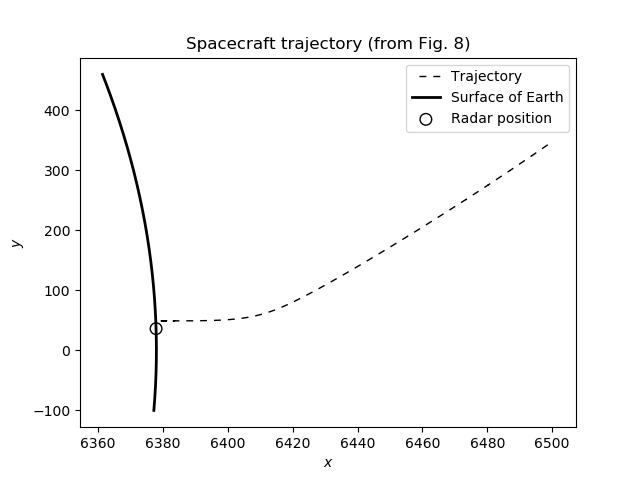
\includegraphics[width=0.95\textwidth]{Fig_8_Trajectory.png}
\captionof{figure}{Trajectory of reentry of a vehicle into the atmosphere of Earth, obtained from equations of motion indicated in \ref{sec:vehicle}. Simulated from Fig. 8 in Julier and Uhlmann\cite{b1}.}
\label{fig:fig8}
\end{figure}

Like in the original paper, we assigned to the system the initial conditions
\[x(0) = \begin{bmatrix} 6500.4 & 349.14 & -1.8093 & -6.7967 & 0.6932 \end{bmatrix}^{T}\]
and
\[P(0) = \begin{bmatrix}
10^{-6} & 0 & 0 & 0 & 0 \\
0 & 10^{-6} & 0 & 0 & 0 \\
0 & 0 & 10^{-6} & 0 & 0 \\
0 & 0 & 0 & 10^{-6} & 0 \\
0 & 0 & 0 & 0 & 0
\end{bmatrix},\]
while we let the unscented Kalman filter assume the initial conditions
\[\mu_{0} = \begin{bmatrix} 6500.4 & 349.14 & -1.8093 & -6.7967 & 0 \end{bmatrix}^{T}\]
and
\[K_{0} = \begin{bmatrix}
10^{-6} & 0 & 0 & 0 & 0 \\
0 & 10^{-6} & 0 & 0 & 0 \\
0 & 0 & 10^{-6} & 0 & 0 \\
0 & 0 & 0 & 10^{-6} & 0 \\
0 & 0 & 0 & 0 & 1
\end{bmatrix},\]
indicating that there is relative initial certainty of the value of every variable except the aerodynamic coefficient. The assumed process noise of the filter was adapted from the actual process noise $v(k)$,
\[Q(k) = \begin{bmatrix}
2.4064 \times 10^{-5} & 0 & 0 \\
0 & 2.4064 \times 10^{-5} & 0 \\
0 & 0 & 0 \end{bmatrix}.\]
The measurements and updates were performed at a frequency of 10 Hz, and the simulation was performed for a duration of 200 seconds, for a total of 1000 iterations.

 For visual reference, we provided a plot of the estimated trajectory of the vehicle, compared to the vehicle's true trajectory, in Fig.~\ref{fig:est_trajectory}. Our results shown in Fig.~\ref{fig:results} are of the mean squared error and variance for the unscented Kalman filter for $x_{1}$, $x_{3}$, and $x_{5}$, which represent the vehicle's $x$-position, $x$-velocity, and aerodynamic coefficient, respectively. We only plotted the error of the mean, as well as the covariance, from the unscented Kalman filter. As seen in Fig.~\ref{fig:est_trajectory}, our Kalman filter implementation tracks the trajectory of the vehicle reasonably well up to the termination of the estimation program, represented by the red \color{red}x \color{black} in the plot. We could not quite replicate the error estimation of the original simulation, likely due to differences in the way we calculated and/or reported our error calculations. This divergence could also be a result of the difference in randomization between the original simulation and our implementation. Nonetheless, our trajectory tracking via unscented Kalman filter has performed similarly well.

\begin{figure}[htb]
\centering\noindent
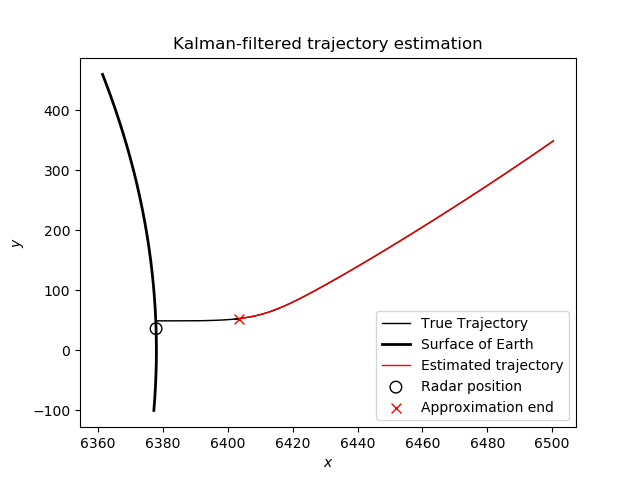
\includegraphics[width=0.95\textwidth]{Estimated_Trajectory.png}
\caption{Result of estimated trajectory versus true trajectory.}
\label{fig:est_trajectory}
\end{figure}

\begin{figure}[ht]
\centering\noindent
\begin{subfigure}{0.48\textwidth}
    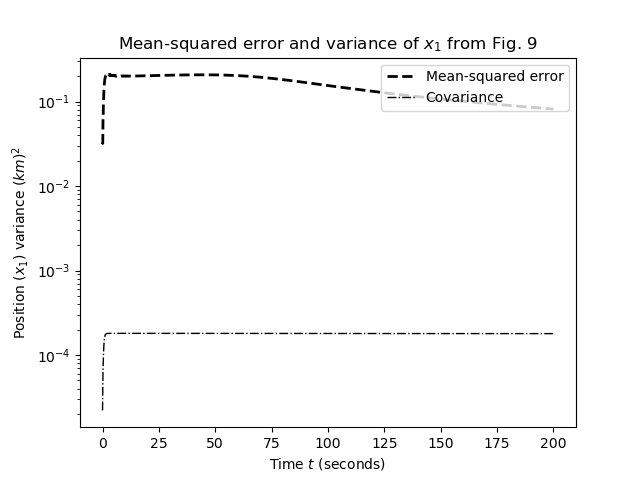
\includegraphics[width=\linewidth, height=5cm]{x1.png}
    \captionof{figure}{Error of mean and covariance of $x_{1}$.}
    \label{fig:results_x1}
\end{subfigure}
\begin{subfigure}{0.48\textwidth}
    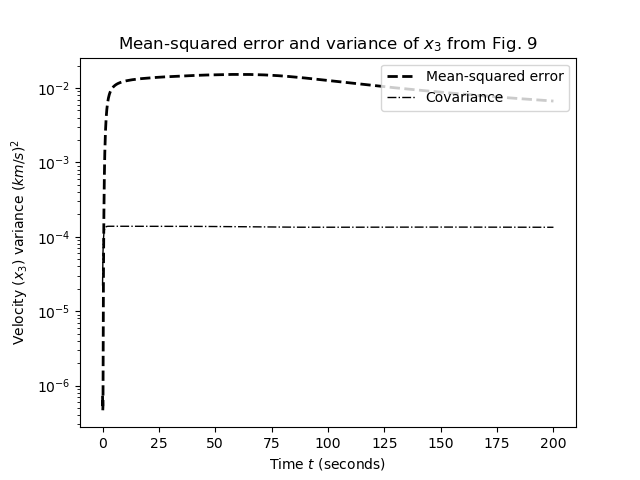
\includegraphics[width=\linewidth, height=5cm]{x3.png}
    \captionof{figure}{Error of mean and covariance of $x_{3}$.}
    \label{fig:results_x3}
\end{subfigure}
\begin{subfigure}{0.48\textwidth}
    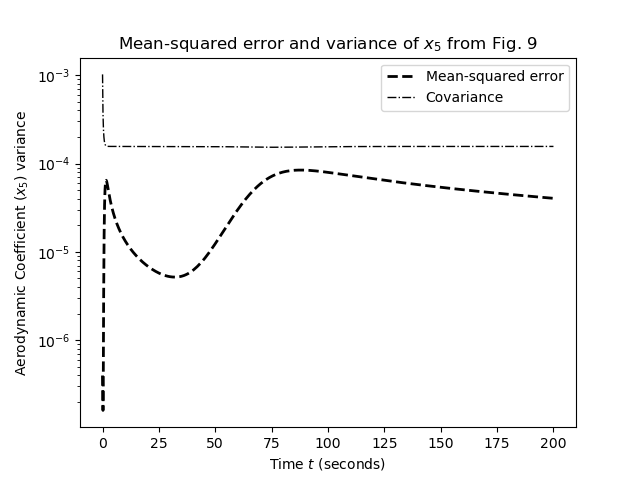
\includegraphics[width=\linewidth, height=5cm]{x5.png}
    \captionof{figure}{Error of mean and covariance of $x_{5}$.}
    \label{fig:results_x5}
\end{subfigure}
\caption{Results of our simulation, as described in section \ref{sec:vehicle}.}
\label{fig:results}
\end{figure}

\section{Conclusion}

This project revolved around the implementation of the unscented Kalman filter for estimation of variables in a nonlinear system with non-Gaussian-distributed noise. Leading to this implementation, we also implemented the standard linear Kalman filter, as well as the extended Kalman filter for nonlinear systems. We also showed a comparison of the linear and unscented Kalman filters with a sinusoidal example in section \ref{sec:sine}. From the original paper by Julier and Uhlmann, we managed to replicate the results of the transformation of statistical data\textemdash mean and covariance\textemdash\ shown in this report in Fig.~\ref{fig:cart_polar} and described in section \ref{sec:cart_polar}. We also managed to replicate results of the vehicle trajectory estimation in section \ref{sec:vehicle}.

\subsection{Future work}

This Kalman filter implementation has room for improvement, as well as potential for further exploration. The primary aspect that can be improved is the separation of the prediction and measurement stages. As of right now, the prediction and measurement steps are alternated continuously. This process can be generalized for the case of multiple predictions between measurements, as well as, conversely, multiple measurements at once. This update would be practically useful for, say, a sensor that provides few measurements far in between, so that the filter would have to continuously estimate the change in the state vector and error covariance matrix before receiving another measurement. Likewise, in practice, a system may have multiple sensors, with inputs possibly arriving simultaneously, in which case one would wish to run the measurement step multiple times in succession before the need to predict future states.

The original paper by Julier and Uhlmann contained some examples of the use of the unscented transform. Replicating more of the results from their work, particularly these unscented transformation examples, would provide more understanding of the uses and limits of the unscented transformation.

Finally, readers who seek to learn more about the situations where various estimation strategies succeed over others would benefit from an extensive direct comparison of the Kalman filters. Theoretical and practical examples utilizing different Kalman filters could be the subject of a future project or report.

\subsection{Acknowledgements}

We would like to thank Dr. Waseem Malik at The University of Maryland, as well as our teaching assistant Srikumar Muralidharan, for giving us a theoretical foundation for completing this project.

\begin{thebibliography}{00}
\bibitem{b1} S. J. Julier, and J. K. Uhlmann, "New extension of the Kalman filter to nonlinear systems," \textit{Proc. SPIE}, vol. 3068, pp. 182-193, July 1997, doi: 10.1117/12.280797.
\bibitem{b2} J. R. R. A. Martins, P. Sturdza, and J. J. Alonso, "The complex-step derivative approximation," \textit{ACM Trans. Math. Softw.}, vol. 29, no. 3, pp. 245-262, Sep. 2003, doi:~10.1145/838250.838251
\bibitem{b3} G. Welch, and G. Bishop, "An introduction to the Kalman filter," Dept. Comp. Sci., Univ. of North Carolina at Chapel Hill, Chapel Hill, NC, USA, Rep. TR 95-041, 2006.

\end{thebibliography}

\end{document}
